% ============================================
% SECTION 2: Methodology
% ============================================
\section{Metodologia}

\begin{frame}{Dataset - Motivação}
    \begin{columns}
    \column{0.5\textwidth}
    \textbf{Datasets Disponíveis}
    \begin{itemize}
        \item PubLayNet, DocLayNet
        \item DocVQA
        \item CORD, SROIE
        \item RVL-CDIP
    \end{itemize}
    \pause
    \column{0.5\textwidth}
    \textbf{RVL-CDIP}
    \begin{itemize}
        \item 400.000 documentos
        \item 16 classes
        \item email, formulário, carta...
        \item Separado por função
    \end{itemize}
\end{columns}
\end{frame}

\begin{frame}{Dataset - Motivação}
    \begin{center}
    \begin{tabular}{@{}ccc@{}}
        \includegraphics[height=0.40\textheight]{images-apresentacao/RVL_EX_1.png} &
        \includegraphics[height=0.40\textheight]{images-apresentacao/RVL_EX_3.png} &
        \includegraphics[height=0.40\textheight]{images-apresentacao/RVL_EX_5.png} \\[0.01cm]
        \includegraphics[height=0.40\textheight]{images-apresentacao/RVL_EX_2.png} &
        \includegraphics[height=0.40\textheight]{images-apresentacao/RVL_EX_4.png} &
        \includegraphics[height=0.40\textheight]{images-apresentacao/RVL_EX_6.png}
    \end{tabular}
    \end{center}
\end{frame}

\begin{frame}{Dataset - Motivação}
    \begin{center}
    \begin{tabular}{@{}ccc@{}}
        \tikz\node[draw=red!80!black,    line width=3pt, inner sep=0pt]{\includegraphics[height=0.40\textheight]{images-apresentacao/RVL_EX_1.png}}; &
        \tikz\node[draw=green!80!black,  line width=3pt, inner sep=0pt]{\includegraphics[height=0.40\textheight]{images-apresentacao/RVL_EX_3.png}}; &
        \tikz\node[draw=blue!80!black,   line width=3pt, inner sep=0pt]{\includegraphics[height=0.40\textheight]{images-apresentacao/RVL_EX_5.png}}; \\[0.01cm]
        \tikz\node[draw=red!80!black,    line width=3pt, inner sep=0pt]{\includegraphics[height=0.40\textheight]{images-apresentacao/RVL_EX_2.png}}; &
        \tikz\node[draw=green!80!black,  line width=3pt, inner sep=0pt]{\includegraphics[height=0.40\textheight]{images-apresentacao/RVL_EX_4.png}}; &
        \tikz\node[draw=blue!80!black,   line width=3pt, inner sep=0pt]{\includegraphics[height=0.40\textheight]{images-apresentacao/RVL_EX_6.png}};
    \end{tabular}
    \end{center}
\end{frame}
    
\begin{frame}{LA-CDIP Dataset - Processo de Rotulação}
\begin{center}
    \includegraphics[height=.8\textheight]{images-apresentacao/clusteringBB.drawio.pdf}
\end{center}
\end{frame}

\begin{frame}{LA-CDIP Dataset - Processo de Rotulação}
\begin{center}
    \includegraphics[width=.8\textwidth]{images-apresentacao/ambiente_publico.drawio.pdf}
\end{center}
\end{frame}

% \begin{frame}{Dataset - Motivação}
%     \begin{center}
%     \begin{tabular}{@{}ccc@{}}
%         \tikz\node[draw=black, line width=2pt, inner sep=0pt]{\includegraphics[height=0.40\textheight]{images-apresentacao/Exemplo_cluster (1).jpg}}; &
%         \tikz\node[draw=black, line width=2pt, inner sep=0pt]{\includegraphics[height=0.40\textheight]{images-apresentacao/Exemplo_cluster (3).jpg}}; &
%         \tikz\node[draw=black, line width=2pt, inner sep=0pt]{\includegraphics[height=0.40\textheight]{images-apresentacao/Exemplo_cluster (5).jpg}}; \\[0.01cm]
%         \tikz\node[draw=black, line width=2pt, inner sep=0pt]{\includegraphics[height=0.40\textheight]{images-apresentacao/Exemplo_cluster (2).jpg}}; &
%         \tikz\node[draw=black, line width=2pt, inner sep=0pt]{\includegraphics[height=0.40\textheight]{images-apresentacao/Exemplo_cluster (4).jpg}}; &
%         \tikz\node[draw=black, line width=2pt, inner sep=0pt]{\includegraphics[height=0.40\textheight]{images-apresentacao/Exemplo_cluster (6).jpg}};
%     \end{tabular}
%     \end{center}
% \end{frame}

\begin{frame}{Visual Document Matching - Ilustração}
\begin{center}
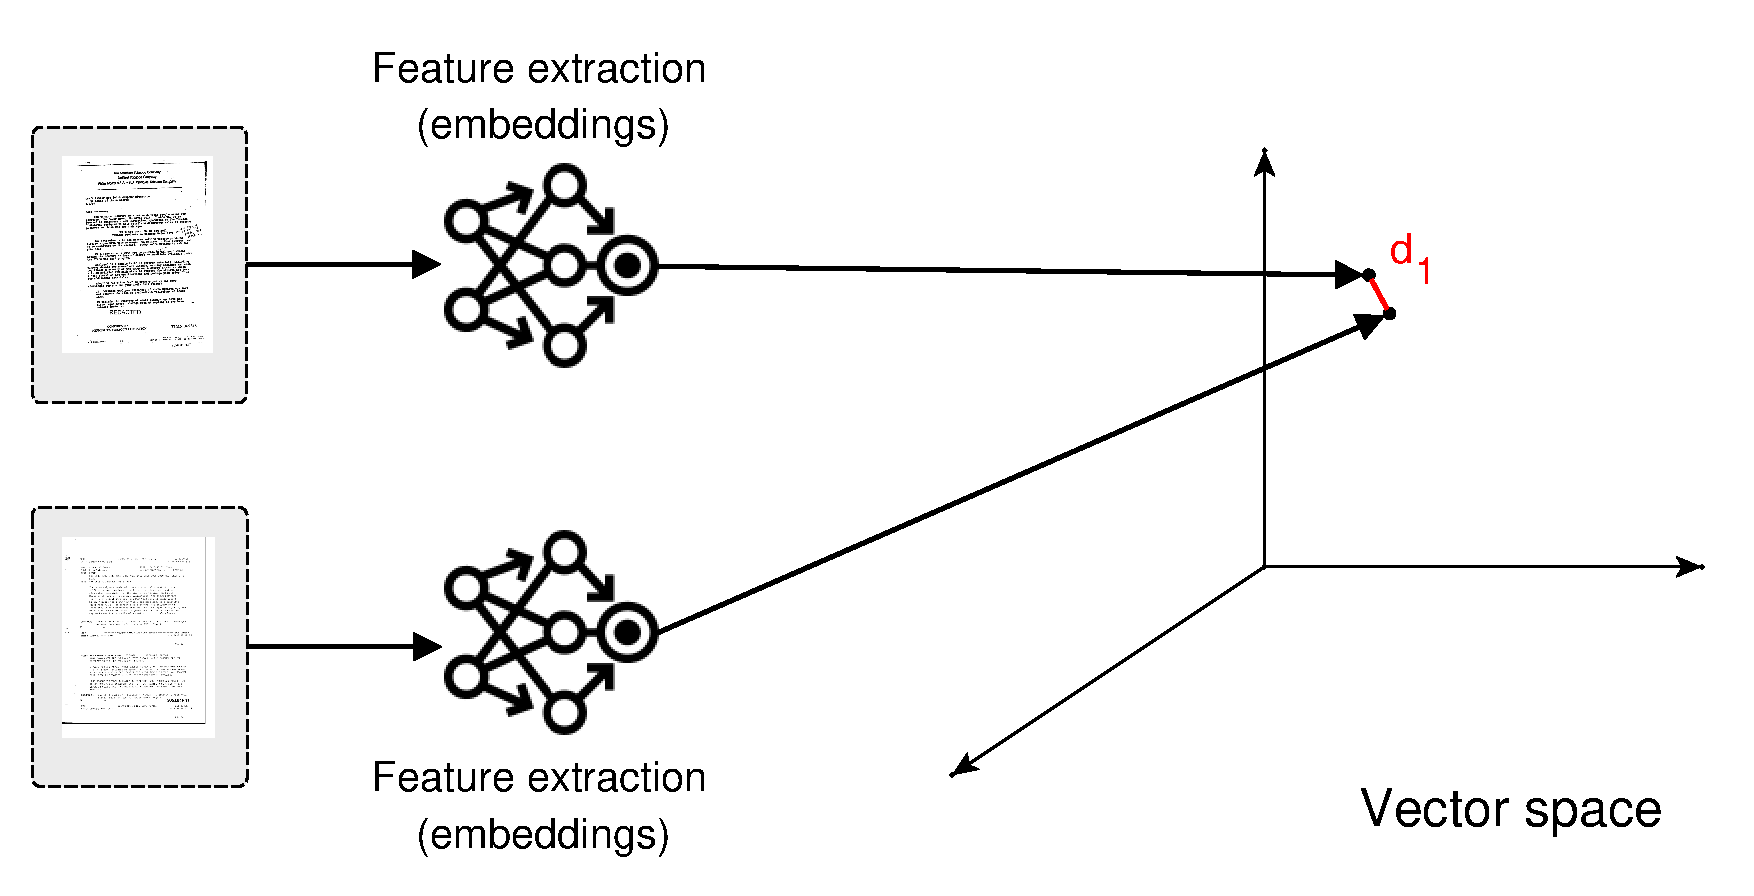
\includegraphics[width=0.8\textwidth]{images/vector_space_1.pdf}
\end{center}
\end{frame}

\begin{frame}{Visual Document Matching - Ilustração}
\begin{center}
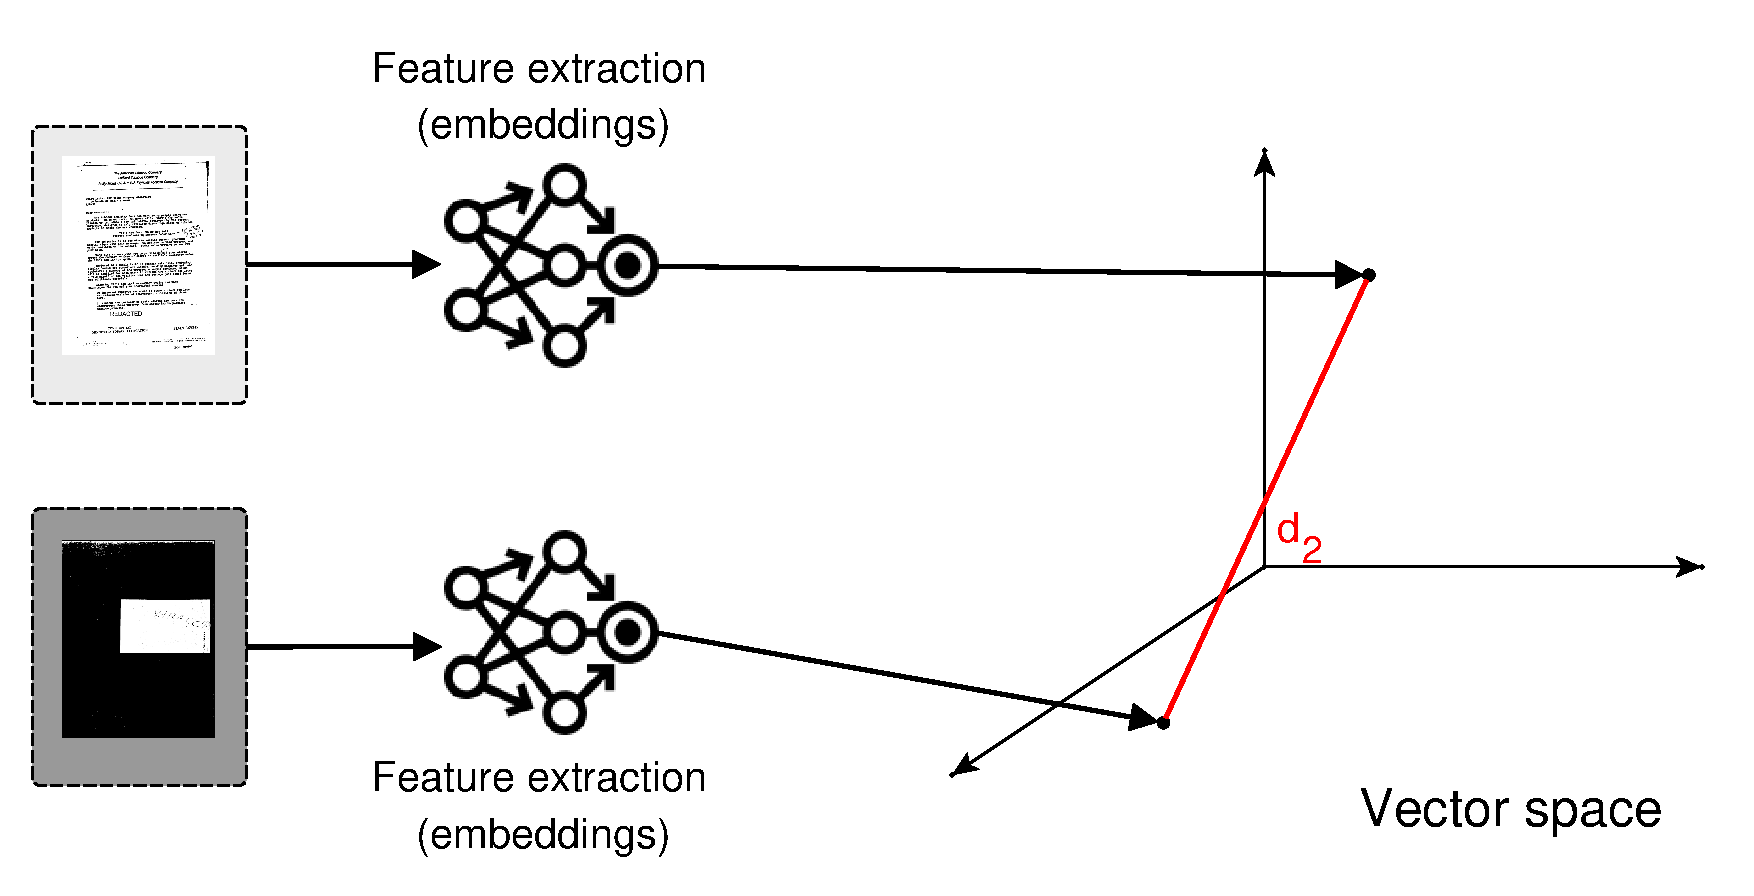
\includegraphics[width=0.8\textwidth]{images/vector_space_2.pdf}
\end{center}
\end{frame}

\begin{frame}{VDM - Arquitetura}
    \begin{columns}
    \column{0.55\textwidth}
    \begin{center}
        \includegraphics[width=\textwidth]{images/siamese.png}
    \end{center}
    
    \column{0.4\textwidth}
    \begin{equation*}
        \mathcal{L} = \begin{cases}
            d(x_1, x_2)^2, & \text{if } y = 1 \\
            (m - d(x_1, x_2))^2, & \text{otherwise}.
    \end{cases}
    \end{equation*}
    \end{columns}
\end{frame}

\begin{frame}{Model Backbone}
\begin{columns}[c]
\column{0.2\textwidth}
\begin{center}
\includegraphics[width=\textwidth]{images-apresentacao/model_backbone.png}
\end{center}

\column{0.1\textwidth}
\begin{center}
{\Huge $\left\{\rule{0pt}{2cm}\right.$}
\end{center}

\column{0.45\textwidth}
\begin{itemize}
    \item AlexNet
    \item ResNet
    \item VGG
    \item EfficientNet
    \item MobileNetV3
    \item Vision Transformer (ViT)
\end{itemize}
\end{columns}
\end{frame}

\begin{frame}{Benchmarking com LLMs}
\begin{columns}
\column{0.5\textwidth}
\textbf{Modelos Avaliados:}
\begin{itemize}
    \item LLaVA 3.2 Vision
    \item InternVL 2.5
    \item Qwen2.5-VL
    \item GPT-4o (2024-11-20)
    \item GPT-4o-mini (2024-07-18)
\end{itemize}

\column{0.5\textwidth}
\textbf{Avaliação:}
\begin{itemize}
    \item Zero-shot (sem fine-tuning)
    \item Pontuação de similaridade 0--100
    \item 5 níveis de categorização
\end{itemize}
\end{columns}
\end{frame}

\begin{frame}{Benchmarking com LLMs - Exemplos}
\begin{columns}
\column{0.5\textwidth}
\begin{center}
\includegraphics[width=\textwidth]{images/similar.png}
\end{center}

\column{0.5\textwidth}
\begin{center}
\includegraphics[width=\textwidth]{images/different.png}
\end{center}
\end{columns}
\end{frame}

